\documentclass[14pt,a4paper]{report}  %紙張設定
\usepackage{xeCJK}%中文字體模組
%\setCJKmainfont{標楷體} %設定中文字體
\setCJKmainfont{MoeStandardKai.ttf}
%\newfontfamily\sectionef{Times New Roman}%設定英文字體
\newfontfamily\sectionef{Nimbus Roman}
\usepackage{enumerate}
\usepackage{amsmath,amssymb}%數學公式、符號
\usepackage{amsfonts} %數學簍空的英文字
\usepackage{graphicx, subfigure}%圖形
\usepackage{fontawesome5} %引用icon
\usepackage{type1cm} %調整字體絕對大小
\usepackage{textpos} %設定文字絕對位置
\usepackage[top=2.5truecm,bottom=2.5truecm,
left=3truecm,right=2.5truecm]{geometry}
\usepackage{titlesec} %目錄標題設定模組
\usepackage{titletoc} %目錄內容設定模組
\usepackage{textcomp} %表格設定模組
\usepackage{multirow} %合併行
%\usepackage{multicol} %合併欄
\usepackage{CJK} %中文模組
\usepackage{CJKnumb} %中文數字模組
\usepackage{wallpaper} %浮水印
\usepackage{listings} %引用程式碼
\usepackage{hyperref} %引用url連結
\usepackage{setspace}
\usepackage{lscape}%設定橫式
\lstset{language=Python, %設定語言
		basicstyle=\fontsize{10pt}{2pt}\selectfont, %設定程式內文字體大小
		frame=lines,	%設定程式框架為線
}
%\usepackage{subcaption}%副圖標
\graphicspath{{./../images/}} %圖片預設讀取路徑
\usepackage{indentfirst} %設定開頭縮排模組
\renewcommand{\figurename}{\Large 圖.} %更改圖片標題名稱
\renewcommand{\tablename}{\Large 表.}
\renewcommand{\lstlistingname}{\Large 程式.} %設定程式標示名稱
\hoffset=-5mm %調整左右邊界
\voffset=-8mm %調整上下邊界
\setlength{\parindent}{3em}%設定首行行距縮排
\usepackage{appendix} %附錄
\usepackage{diagbox}%引用表格
\usepackage{multirow}%表格置中
%\usepackage{number line}
%=------------------更改標題內容----------------------=%
\titleformat{\chapter}[hang]{\center\sectionef\fontsize{20pt}{1pt}\bfseries}{\LARGE 第\CJKnumber{\thechapter}章}{1em}{}[]
\titleformat{\section}[hang]{\sectionef\fontsize{18pt}{2.5pt}\bfseries}{{\thesection}}{0.5em}{}[]
\titleformat{\subsection}[hang]{\sectionef\fontsize{18pt}{2.5pt}\bfseries}{{\thesubsection}}{1em}{}[]
%=------------------更改目錄內容-----------------------=%
\titlecontents{chapter}[11mm]{}{\sectionef\fontsize{18pt}{2.5pt}\bfseries\makebox[3.5em][l]
{第\CJKnumber{\thecontentslabel}章}}{}{\titlerule*[0.7pc]{.}\contentspage}
\titlecontents{section}[18mm]{}{\sectionef\LARGE\makebox[1.5em][l]
{\thecontentslabel}}{}{\titlerule*[0.7pc]{.}\contentspage}
\titlecontents{subsection}[4em]{}{\sectionef\Large\makebox[2.5em][l]{{\thecontentslabel}}}{}{\titlerule*[0.7pc]{.}\contentspage}
%=----------------------章節的間距----------------------=%
\titlespacing*{\chapter} {0pt}{0pt}{18pt}
\titlespacing*{\section} {0pt}{12pt}{6pt}
\titlespacing*{\subsection} {0pt}{6pt}{6pt}
%=----------------------標題-------------------------=%             
\begin{document} %文件
\sectionef %設定英文字體啟用
\vspace{12em}
\begin{titlepage}%開頭
\begin{center}   %標題  
\makebox[1.5\width][s] %[s] 代表 Stretch the interword space in text across the entire width
{\fontsize{24pt}{2.5pt}國立虎尾科技大學}\\[18pt]
\makebox[1.5\width][s]
{\fontsize{24pt}{2.5pt}機械設計工程系}\\[18pt]
\sectionef\fontsize{24pt}{1em}\selectfont\textbf
{
\vspace{0.5em}
cd2023 2b-pj2bg7分組報告}\\[18pt]
%設定文字盒子 [方框寬度的1.5倍寬][對其方式為文字平均分分布於方框中]\\距離下方18pt
\vspace{1em} %下移
\fontsize{30pt}{1pt}\selectfont\textbf{網際足球場景設計}\\
\vspace{1em}
\sectionef\fontsize{30pt}{1em}\selectfont\textbf
{
\vspace{0.5em}
Web-based Football Scene Design}
 \vspace{2em}
%=---------------------參與人員-----------------------=%             
\end{center}
\begin{flushleft}
\begin{LARGE}

\hspace{32mm}\makebox[5cm][s]
{指導教授:\quad 嚴\quad 家\quad 銘\quad 老\quad 師}\\[6pt]
\hspace{32mm}\makebox[5cm][s]
{班\qquad 級:\quad 四\quad 設\quad 二\quad 乙}\\[6pt]
\hspace{32mm}\makebox[5cm][s]
{學\qquad 生:\quad 陳\quad 冠\quad 珉\quad(41023220)}
\\[6pt]
\hspace{32mm}\makebox[5cm][s]
{\hspace{36.5mm}陳\quad 建\quad 霖\quad(41023226)}\\[6pt]
\hspace{32mm}\makebox[5cm][s]
{\hspace{36.5mm}黃\quad 文\quad 彥\quad(41023233)}\\[6pt]
\hspace{32mm}\makebox[5cm][s]
{\hspace{36.5mm}謝\quad 宗\quad 銘\quad(41023253)}\\[6pt]
\hspace{32mm}\makebox[5cm][s]

%設定文字盒子[寬度為5cm][對其方式為文字平均分分布於方框中]空白距離{36.5mm}\空白1em
\end{LARGE}
\end{flushleft}
\vspace{6em}
\fontsize{18pt}{2pt}\selectfont\centerline{\makebox[\width][s]
{中華民國\hspace{3em} 
112 \quad 年\quad 5\quad 月}}
\end{titlepage}
\newpage

%=------------------------摘要-----------------------=%
\renewcommand{\baselinestretch}{1.5} %設定行距
\pagenumbering{roman} %設定頁數為羅馬數字
\clearpage  %設定頁數開始編譯
\sectionef
\addcontentsline{toc}{chapter}{摘~~~要} %將摘要加入目錄
\begin{center}
\LARGE\textbf{摘~~要}\\
\end{center}
\begin{flushleft}
\fontsize{14pt}{20pt}\sectionef\hspace{12pt}\quad 專案二的目標是進行協同設計,將雙輪車應用於機器人足球比賽中。團隊組成包含4名成員,使用CAD軟體進行場景和雙輪車零組件的設計。專案的主要焦點是在足球場景中控制雙輪車進行比賽,並確保每組有4名輪車球員參與比賽。\\[12pt]

\fontsize{14pt}{20pt}\sectionef\hspace{12pt}\quad 此外,團隊還將設計單機記分板,以便在比賽中追蹤並顯示比分。記分板將使用LED顯示器來顯示分數,以便參與者和觀眾能夠隨時瞭解比賽的進展。\\[12pt]

\end{flushleft}
\begin{center}
\fontsize{14pt}{20pt}\selectfont 透過專案二的協同設計,團隊將有機會實踐協同工作並應用雙輪車於足球比賽。這將提供團隊成員們在實際場景中運用他們的技術和創造力的機會,同時為未來的機器人足球比賽項目提供基礎和啟示。
\end{center}
\newpage
%=--------------------Abstract----------------------=%
\newpage
\renewcommand{\baselinestretch}{1.5} %設定行距

%=------------------------誌謝----------------------=%
\begin{center}	
\addcontentsline{toc}{chapter}{誌~~~謝}
\LARGE\textbf{誌~~謝}\\
\end{center}
\begin{center}
\begin{flushleft}
\fontsize{14pt}{20pt}\sectionef\hspace{12pt}\quad 在此鄭重感謝製作以及協助本分組報告完成的所有人員,首先向嚴家銘老師致謝,他解決我們的各種提問,甚至從來沒有不耐煩,總是貼心為我們找出最佳解答,接著是由OpenAI創造的ChatGPT,在我們需要創作的時候,他總能提供我們源源不斷的創意,最後是由本分組成員同心協力才得以完成本報告,特此感謝

\end{flushleft}
\newpage
%=------------------------目錄----------------------=%
\renewcommand{\contentsname}{\centerline{\fontsize{18pt}{\baselineskip}\selectfont\textbf{目\quad 錄}}}
\tableofcontents  %目錄產生
\newpage

\end{center}
%=-------------------------內容----------------------=%

\chapter{更新團隊網站步驟}
\section{詳細步驟說明}


 1.先開起個人USB中的倉儲ipv6\\

2.在至個人github中的fork倉儲更新成最新版\\

3.輸入git pull若失敗則有可能PUTTY跑掉重設定即可\\

4.進行編輯\\

5.acp\\

6.在至個人fork倉儲Open pull request\\

7.若無法pull request 那就至個人fork在合併最新版本並除錯即可\\

8.一路同意推送合併到底\\

9.回到整組倉儲確認上傳己完成\\




\chapter{W9}


\section{W9\_41023220}

心得:今天對removeAPI有了初步的認知,覺得自己可以做得更好。

\section{W9\_41023226}

心得:今天使用老師給的removeAPI的程式控制機器人,可以透過改IP的方式操控其他電腦的機器人,十分有趣。

\section{W9\_41023233}

心得:今天使用了老師給的資料夾bubbleRob_zmq_green_red_example開啟了coppelia,學習到怎麼操控機器人。

\section{W9\_41023253}

心得:今天跟著老師嘗試進行了removeAPI,讓我對IP控制有了初步的概念了,希望未來能夠順利地跟上課程。


\chapter{W10}
\section{第一題}
What is zmqRemoteAPI, and how does it relate to CoppeliaSim?

答

 zmqRemoteAPI 是一種遠端 API(應用程式編程介面),允許使用外部編寫的程式(例如 Python、C++ 或 Matlab)連接到機器人模擬軟體 CoppeliaSim。zmqRemoteAPI 使用 ZeroMQ 網路庫進行通訊,讓使用者能夠即時互動仿真環境。


\section{第二題}
How do you establish a connection between a Python script and CoppeliaSim using zmqRemoteAPI?

答

python先下載zmq子模組,利用port:23000連接


\section{第三題}
What are some common use cases for zmqRemoteAPI in CoppeliaSim?

答

在 CoppeliaSim 中使用 zmqRemoteAPI 的一些常見用例包括:

機器人模擬的即時控制
資料收集和分析
仿真資料的可視化
控制演算法的測試和驗證


\section{第四題}
What are the advantages and disadvantages of using zmqRemoteAPI compared to other methods of communication between Python and CoppeliaSim?

答

快速高效的通訊
支援多種程式語言
即時互動仿真環境
允許遠端存取仿真
缺點可能包括更陡峭的學習曲線和需要額外的程式庫。

相較於其他通訊方法,使用 zmqRemoteAPI 需要較多的程式設計經驗和了解 ZeroMQ 網路庫的概念。另外,使用 zmqRemoteAPI 需要安裝和配置 ZeroMQ 網路庫,這可能需要額外的時間和資源。

\section{第五題}
Can you give an example of a project or task that you could complete using zmqRemoteAPI in CoppeliaSim?

答

使用 zmqRemoteAPI,可以在 CoppeliaSim 中完成許多專案或任務。以下是一個使用 zmqRemoteAPI 在 CoppeliaSim 中進行視覺感知的範例:

假設有一個機器人模型,可以透過 CoppeliaSim 遠端 API 伺服器控制。此外,模型上有一個攝影機,可以捕捉模擬環境中的影像。目標是讓機器人模型能夠偵測影像中的物體並移動到它們的位置。

以下是一個使用 Python 和 zmqRemoteAPI 實現的範例:

1.在 CoppeliaSim 中建立一個機器人模型和一個攝影機。

2.在 Python 中使用 zmqRemoteAPI 建立連接,並使用 "simxGetObjectHandle" 函數獲取模型和攝影機的句柄。

3.使用 "simxGetVisionSensorImage" 函數獲取攝影機的畫面。

4.使用 OpenCV 或其他圖像處理程式庫分析攝影機畫面,偵測物體的位置。

5.使用 "simxSetJointTargetPosition" 函數控制機器人模型的移動,使其移動到偵測到的物體的位置。




\section{小組工作分配}
41023219: 

在旁邊研究Brython程式環境

41023228: 

討論與設計程式,製作亂數。
\section{2b網站順序亂數}
\begin{lstlisting}[language=Python, frame=single, numbers=left, captionpos=b, basicstyle=\ttfamily\small, showstringspaces=false, breaklines=true, tabsize=4, xleftmargin=15pt]
from browser import html, document
import random
bcd_tem = "https://mdecd2023.github.io/2b2-pj2bg"
bgithub = "https://github.com/mdecd2023/2b2-pj2bg"
brython_div = document["brython_div1"]
#  亂數範圍從1到16
grp = []
for i in range(1, 17):
    grp.append(i)
random.shuffle(grp)
for i in grp:
    url = bcd_tem + str(i)
    github = bgithub + str(i)
    brython_div <= html.A("pj2bg"+str(i), href=url)
    brython_div <= " ("
    brython_div <= html.A("repo", href=github)
    brython_div <= ")"
    brython_div <= html.BR()
\end{lstlisting}

41023221: 

跟組長一起討論以及改善關於Brython程式的問題

41023222: 

試著幫組長找尋亂數採樣無法正常執行的原因,試著採用其他方法。


\chapter{W11}


\section{41023220}

負責部分:跟組長一起討論作業的開發內容並實測,並教導其他不熟悉的組員\\過程:上次只有把單純的足球場做出來,並沒有計分的規則,在做出記分板以及在寫記分板的程式的時候遇到了不少的問題,但我們都一一克服了\\自評:這次的分組讓我學會了如何解決上傳合併的衝突,然後在修改計分系統的時候遇到了一些問題,很感謝組長的協助。\\自評分數:62分


\section{41023226}

負責部分: 將他們fork後pull request 發生問題時(例:無法auto-merge),負責修改錯誤文件並使其能成功合併、足球場繪製、單機計分板程式設計、做出 PDF 報告\\遇到的難題和心得

1.將計分板程式弄上去後發現球進不會感應,但機器人會,原本以為我的程式出現錯誤,但沒想到是球與機器人的 Collidable(可碰撞) Measurable(可测量) Detectable(可檢測) 設定有誤,應將球的勾選而不是機器人

2.打算將進球後進球方與被進球方放回原位,並將球放在離被進球方較近的位置,結果對 'sim.getObjectPosition' 函數的未知鬧出許多笑話,像是 -1 不知道要放在座標前面還是後面XD

3. 原本打算一開始球以亂數形式產生(避免在正中間而造成雙方僵持不下),但我的記分板中的程式由於第二點以至於一開始一定要有一顆球,而不能我想到的(放進zmq程式中亂數產球)而不了了之,希望之後我能想出個好方法。

4.控制手感是真的差\\自評:遇到需多困境與難題,所幸最後都能有所收穫。\\自評分數:85分

\section{41023233}

負責部分:與組長一起設計球場,還有記分板與程式的設置\\自評:一開始有遇到問題,但是藉由組長組員一起討論還有問別人後,問題有解決\\自評分數:60分


\section{41023253}

負責部分:球門繪製\\心得:在這次的協同作業裡我利用onshape繪製球門場景,從這次作業裡我更加認識了zmqRemoteApi實作的重要性,雖然在計分板場景中因還不熟悉細部操作於是先在旁研究組長是如何做出和除錯的。\\自評分數:60分

%=---------------------參考文獻----------------------=%

%=---------------附錄-----------------=%
\addcontentsline{toc}{chapter}{附錄} %新增目錄名稱

\newpage
%=-------------作者簡介-----------------=%
    \addcontentsline{toc}{chapter}{作者簡介}
    \begin{center}
	\fontsize{20pt}{0em}\selectfont \bf{作者簡介}\\
	\end{center}	
	{\begin{textblock}{6}(0,0.5)
	\begin{figure}
	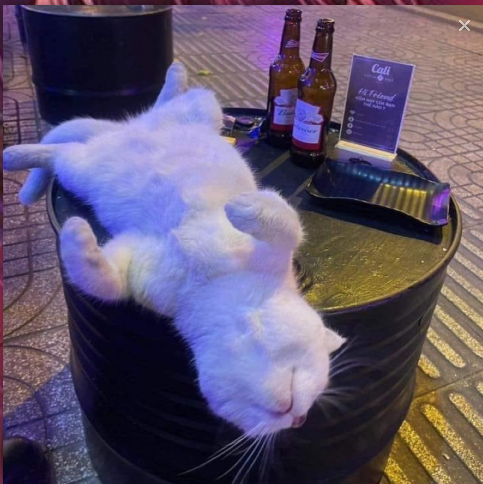
\includegraphics[width=1.25in]{41023220}  %作者照片
	\end{figure}
	\end{textblock}}
	{\renewcommand\baselinestretch{0.99}\selectfont %設定以下行距
	{\begin{textblock}{15}(3.5,0.7)%{寬度}(以左上角為原點之右移量,下移量)
	\noindent\fontsize{14pt}{0em}\selectfont \makebox[4em][s]{姓名}\enspace:\enspace
    \fontsize{14pt}{0em}\selectfont \makebox[4em][s]{陳冠珉}\\     \hspace*{\fill} \\
    \fontsize{14pt}{0em}\selectfont \makebox[4em][s]{學號}\enspace:\enspace
    \fontsize{14pt}{0em}\selectfont \makebox[4em][s]{41023220} \\ %\makebox為文本盒子
    \hspace*{\fill} \\
    \fontsize{14pt}{0em}\selectfont \makebox[4em][s]{就讀學校}\enspace:\enspace
    \fontsize{14pt}{0em}\selectfont \makebox[9em][s]{國立虎尾科技大學}\\
    \fontsize{14pt}{0em}\selectfont \makebox[5em][s]{\quad}\enspace\enspace
    \fontsize{14pt}{0em}\selectfont \makebox[8em][s]{機械設計工程系}\\
    \hspace*{\fill} \\
    \fontsize{14pt}{0em}\selectfont \makebox[4em][s]{經歷}\enspace:\enspace
    \end{textblock}}}
   % \hspace*{\fill} \\
   \vspace{2em}
	{\begin{textblock}{6}(0,2.3)
	\begin{figure}
	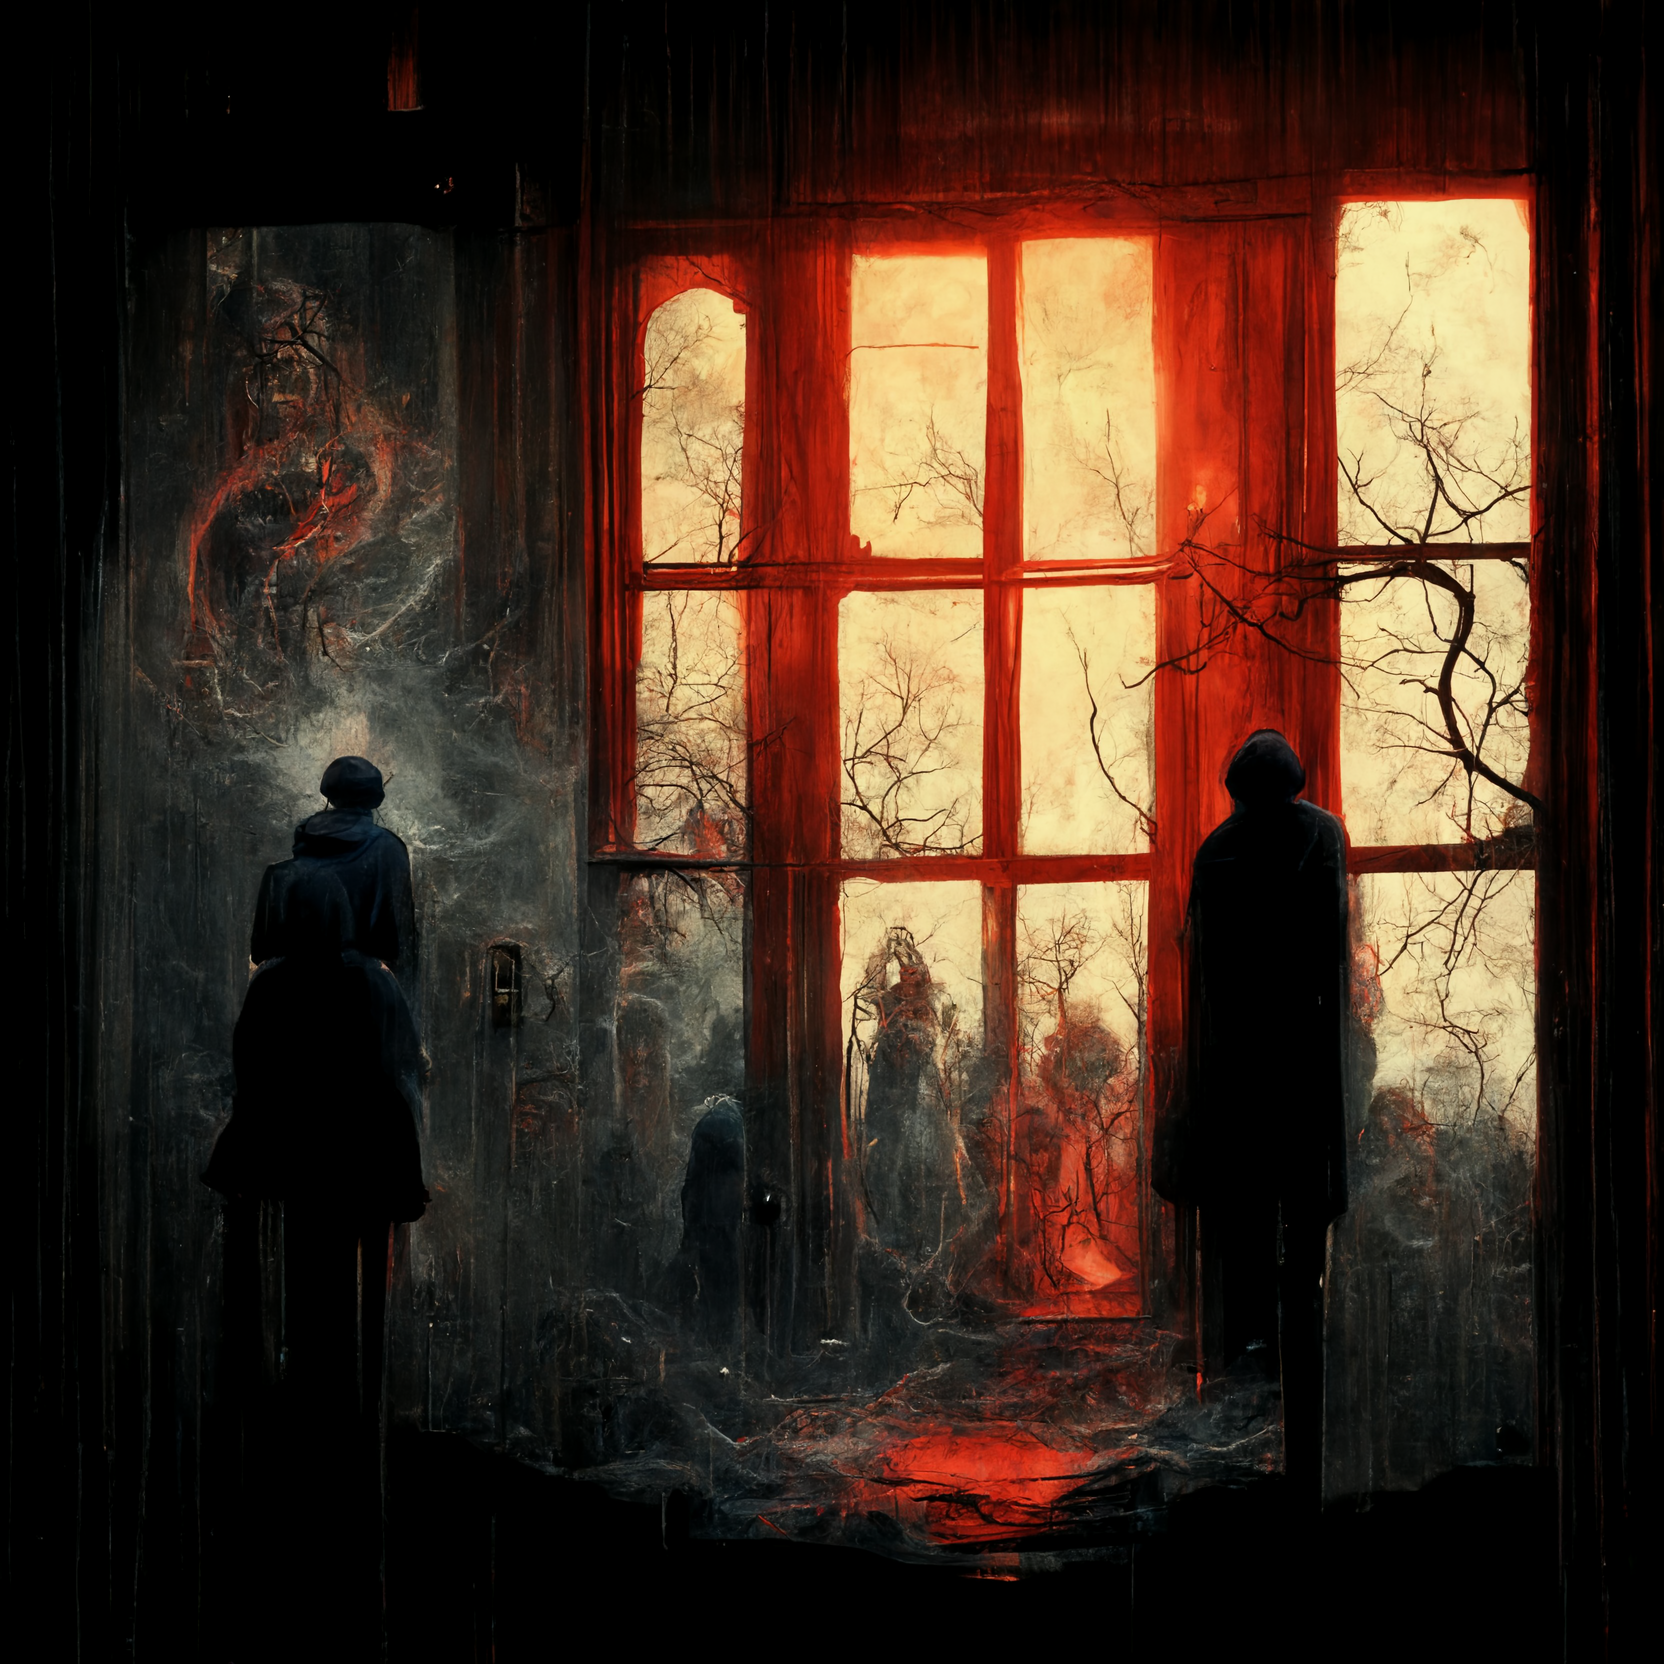
\includegraphics[width=1.15in]{41023226}  %作者照片
    \end{figure}
    \end{textblock}}
    {\renewcommand\baselinestretch{0.99}
    \selectfont %設定以下行距
    {\begin{textblock}{15}(3.5,2.5) %{寬度}(以左上角為原點之右移量,下移量)
\noindent\fontsize{14pt}{0em}\selectfont \makebox[4em][s]{姓名}\enspace:\enspace
\fontsize{14pt}{0em}\selectfont \makebox[4em][s]{陳建霖}\\ 
\hspace*{\fill} \\
\fontsize{14pt}{0em}\selectfont \makebox[4em][s]{學號}\enspace:\enspace
\noindent\fontsize{14pt}{0em}\selectfont \makebox[4em][s]{41023226} \\ 
\hspace*{\fill} \\
\fontsize{14pt}{0em}\selectfont \makebox[4em][s]{就讀學校}\enspace:\enspace
\fontsize{14pt}{0em}\selectfont \makebox[9em][s]{國立虎尾科技大學}\\
\fontsize{14pt}{0em}\selectfont \makebox[5em][s]{\quad}\enspace\enspace
\fontsize{14pt}{0em}\selectfont \makebox[8em][s]{機械設計工程系}\\
\hspace*{\fill} \\
\fontsize{14pt}{0em}\selectfont \makebox[4em][s]{經歷}\enspace:\enspace
    \end{textblock}}}
    %\hspace*{\fill} \\
    \vspace{2em}
    {\begin{textblock}{6}(0,4.1)
    \begin{figure}
        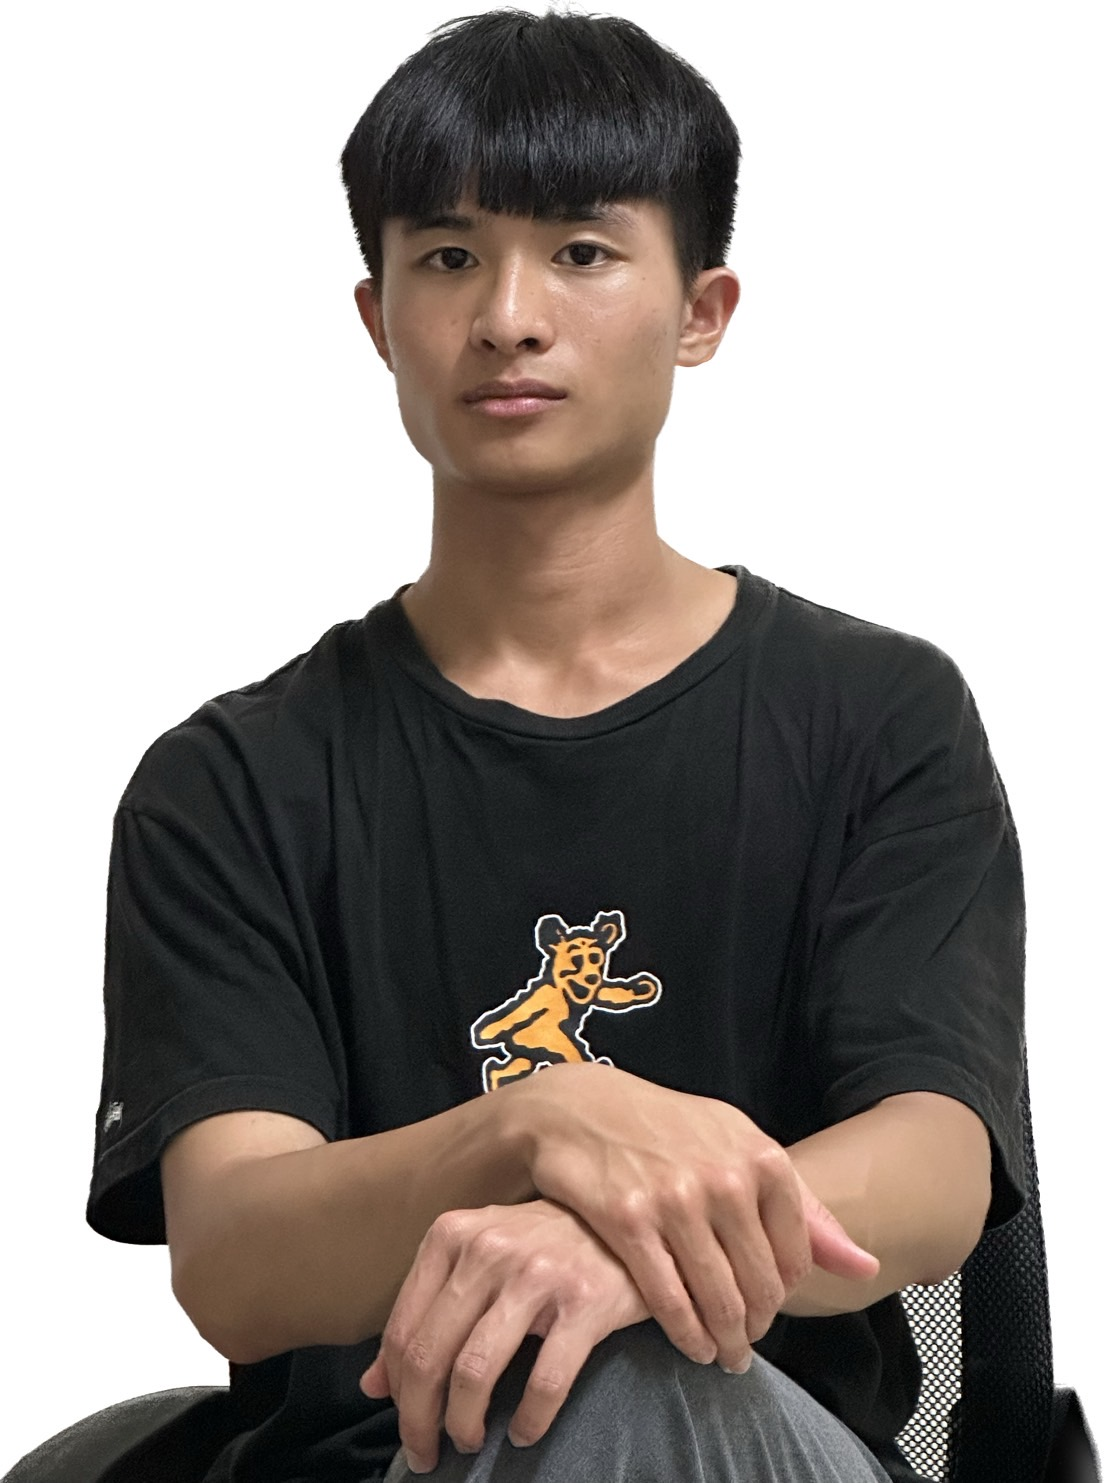
\includegraphics[width=1.15in]{41023233} %{}內是圖片文件的相對路徑
    \end{figure}
    \end{textblock}}
    {\renewcommand\baselinestretch{0.99}\selectfont %設定以下行距
    {\begin{textblock}{15}(3.5,4.3) %{寬度}(以左上角為原點之右移量,下移量)
\noindent\fontsize{14pt}{0em}\selectfont \makebox[4em][s]{姓名}\enspace:\enspace%\noindent指定首行不進行縮排
\fontsize{14pt}{0em}\selectfont \makebox[4em][s]{黃文彥}\\ 
\hspace*{\fill} \\
\noindent\fontsize{14pt}{0em}\selectfont \makebox[4em][s]{學號}\enspace:\enspace
\noindent\fontsize{14pt}{0em}\selectfont \makebox[4em][s]{41023233} \\ %\makebox為文本盒子
\hspace*{\fill} \\
\noindent\fontsize{14pt}{0em}\selectfont \makebox[4em][s]{就讀學校}\enspace:\enspace
\noindent\fontsize{14pt}{0em}\selectfont \makebox[9em][s]{國立虎尾科技大學}\\
\noindent\fontsize{14pt}{0em}\selectfont \makebox[5em][s]{\quad}\enspace\enspace
\noindent\fontsize{14pt}{0em}\selectfont \makebox[8em][s]{機械設計工程系}\\
\hspace*{\fill} \\
\noindent\fontsize{14pt}{0em}\selectfont \makebox[4em][s]{經歷}\enspace:\enspace
    \end{textblock}}}
   % \hspace*{\fill} \\
   \vspace{2em}
    {\begin{textblock}{6}(0,5.9)
    \begin{figure}
        
\includegraphics[width=1.15in]{41023253} %{}內是圖片文件的相對路徑
    \end{figure}
    \end{textblock}}
    {\renewcommand\baselinestretch{0.99}\selectfont %設定以下行距
    {\begin{textblock}{15}(3.5,6.1) %{寬度}(以左上角為原點之右移量,下移量)
\noindent\noindent\fontsize{14pt}{0em}\selectfont \makebox[4em][s]{姓名}\enspace:\enspace
\noindent\fontsize{14pt}{0em}\selectfont \makebox[4em][s]{謝宗銘}\\ \hspace*{\fill} \\
\noindent\fontsize{14pt}{0em}\selectfont \makebox[4em][s]{學號}\enspace:\enspace
\noindent\fontsize{14pt}{0em}\selectfont \makebox[4em][s]{41023253} \\ \hspace*{\fill} \\
\noindent\fontsize{14pt}{0em}\selectfont \makebox[4em][s]{就讀學校}\enspace:\enspace
\noindent\fontsize{14pt}{0em}\selectfont \makebox[9em][s]{國立虎尾科技大學}\\
\noindent\fontsize{14pt}{0em}\selectfont \makebox[5em][s]{\quad}\enspace\enspace
\noindent\fontsize{14pt}{0em}\selectfont \makebox[8em][s]{機械設計工程系}\\
\hspace*{\fill} \\
\noindent\fontsize{14pt}{0em}\selectfont \makebox[4em][s]{經歷}\enspace:\enspace
    \end{textblock}}}
    %\hspace*{\fill} \\

\newpage
%=----------------書背----------------------=%
\pagestyle{empty}%設定沒有頁眉和頁腳
\begin{center}
\fontsize{0.001pt}{1pt}\selectfont .\\
\vspace{4em}
\fontsize{30pt}{30pt}\selectfont 【13】 \\
\fontsize{20pt}{20pt}\selectfont
\vspace{0.5em}
分\\
類\\
編\\
號\\
\vspace{0.5em}
\hspace{-0.5em}:\\
\vspace{0.5em}
\rotatebox[origin=cc]{270}{\sectionef\LARGE \textbf{pj2bg6}}\\ %旋轉
\vspace{0.5em}
網\\
際\\
足\\
球\\
場\\
景\\
設\\
計\\
\vspace{2em}
一\\
一\\
二\\
級\\

\end{center}
%\newpage
%\begin{landscape}  %橫式環境
%\begin{center}
%\fontsize{0.001pt}{1pt}\selectfont .
%\vspace{70mm}
%\rotatebox[origin=cc]{90}{\LARGE 【14】}\rotatebox[origin=cc]%{180}{\LARGE 1-2-APP-8765} %旋轉
%\end{center}
%\end{landscape}
\end{document}
